\newcommand{\psd}[1]{{\small\sffamily{\color{blue!60}#1}}}

\begin{figure}[h!]
\centering
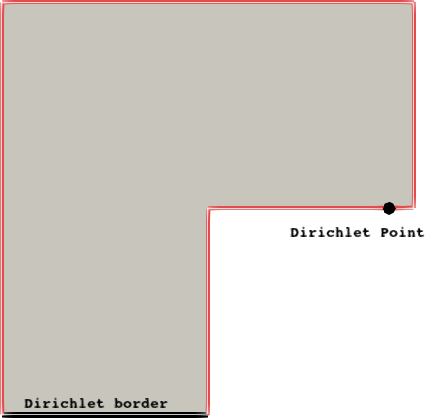
\includegraphics[width=0.3\textwidth]{./Images/fm-geometry.png}
\caption{Geometry of the L-shaped test used in this tutorial. \label{L-shape-geo}}
\end{figure}

\subsection{Preprocessing}

You can either solver the problem using vectorial approach (recommended)
or using staggered approach. To generate the solver use either from
below.

\textbf{Generation of solver (vectorial)}

\begin{lstlisting}[style=BashInputStyle]
PSD_PreProcess -dimension 2 -problem damage -model hybrid_phase_field \
-dirichletconditions 1 -dirichletpointconditions 1 -debug -postprocess ud \
-energydecomp -constrainHPF -vectorial -getreactionforce -plotreactionforce \
-reactionforce variational_based
\end{lstlisting}

\textbf{Generating solver (staggered)}

\begin{lstlisting}[style=BashInputStyle]
PSD_PreProcess -dimension 2 -problem damage -model hybrid_phase_field \
-dirichletconditions 1 -dirichletpointconditions 1 -debug -postprocess ud \
-energydecomp -constrainHPF -getreactionforce -plotreactionforce \
-reactionforce variational_based
\end{lstlisting}

\subsection{Edit Cycle}

\textbf{Edit ControlParameter.edp:}

\begin{itemize}

\item Update physical parameter, change

\begin{lstlisting}[style=CppStyle]
  real lambda = 121.15e3 ,
       mu     = 80.77e3  ,
       Gc     = 2.7      ;
\end{lstlisting}

to

\begin{lstlisting}[style=CppStyle]
  real lambda = 6.16e3 ,
       mu     = 10.95e3 ,
       Gc     = 8.9e-2  ;
\end{lstlisting}

\item Update solver parameter , change

\begin{lstlisting}[style=CppStyle]
  real lfac  = 2.0  ,
       maxtr = 7e-3 ,
       tr    = 1e-5 ,
       dtr   = 1e-5 ,
       lo           ;
\end{lstlisting}

to

\begin{lstlisting}[style=CppStyle]
  real lfac  = 2.0  ,
       maxtr = 1    ,
       tr    = 1e-2 ,
       dtr   = 1e-2 ,
       lo           ;
\end{lstlisting}


\item Enter the correct Point boundary condition, change

\begin{lstlisting}[style=CppStyle]
  real[int,int] PbcCord = [
//-------------------- [  x  , y  ] --------------------//
                       [  0. , 0. ]    // point 0
//------------------------------------------------------//
                      ];

   macro Pbc0Ux  -0. //
   macro Pbc0Uy  -0. //
\end{lstlisting}

to

\begin{lstlisting}[style=CppStyle]
  real[int,int] PbcCord = [
//-------------------- [  x  , y  ] --------------------//
                       [  470., 250. ]    // point 0
//------------------------------------------------------//
                      ]
;
   macro Pbc0Uy  tr //
\end{lstlisting}

\end{itemize}

\textbf{Edit LinearFormBuilderAndSolver.edp:}

\begin{itemize}

\item To postprocess correct reaction forces in LinearFormBuilderAndSolver.edp for vectorial solver, change

\begin{lstlisting}[style=CppStyle]
  for(int i=0; i < Th.nv; i++){
     if(abs(Th(i).y-1.)<.000001){
        forcetotx = forcetotx + F[][i*3]*DP[i*3];
        forcetoty = forcetoty + F[][i*3+1]*DP[i*3+1];
     }
  }
\end{lstlisting}

to

\begin{lstlisting}[style=CppStyle]
  if(mpirank==mpirankPCi[0]){
     forcetotx = forcetotx + F[][PCi[0]*3+0]*DP[PCi[0]*3+0];
     forcetoty = forcetoty + F[][PCi[0]*3+1]*DP[PCi[0]*3+1];
  }
\end{lstlisting}

\item To postprocess correct reaction forces in LinearFormBuilderAndSolver.edp for staggered solver, change

\begin{lstlisting}[style=CppStyle]
  for(int i=0; i < Th.nv; i++){
     if(abs(Th(i).y-1.)<.000001){
        forcetotx = forcetotx + F[][i*2]*DP[i*2];
        forcetoty = forcetoty + F[][i*2+1]*DP[i*2+1];
     }
  }
\end{lstlisting}

to

\begin{lstlisting}[style=CppStyle]
  if(mpirank==mpirankPCi[0]){
     forcetotx = forcetotx + F[][PCi[0]*2+0]*DP[PCi[0]*2+0];
     forcetoty = forcetoty + F[][PCi[0]*2+1]*DP[PCi[0]*2+1];
  }
\end{lstlisting}

\item Finally to include cyclic loading, change

\begin{lstlisting}[style=CppStyle]
  //-----------------updating traction----------------//

  tr += dtr;
\end{lstlisting}


to

\begin{lstlisting}[style=CppStyle]
  //-----------------updating traction----------------//

  if(iterout<50)
     tr += dtr;
  if(iterout>=51 && iterout<110)
     tr -= dtr;
  if(iterout>=111)
     tr += dtr;
\end{lstlisting}

\begin{figure}[h!]
\centering
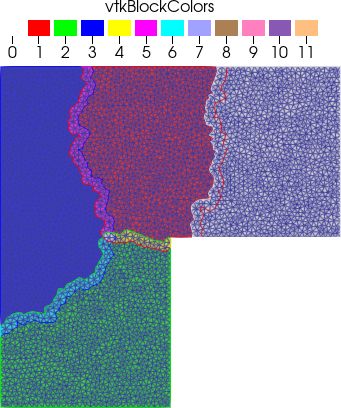
\includegraphics[width=0.3\textwidth]{./Images/fm-mesh.png}
\caption{Finite element mesh of the L-shaped test. \label{L-shape-mesh}}
\end{figure}

\end{itemize}

\subsection{Solving}

Irrespective of weather vectorial or staggered mode is used solve the
problem using \psd{PSD\_Solve}

\begin{lstlisting}[style=BashInputStyle]
PSD_Solve -np 4 Main.edp -wg -v 0 -mesh ./../Meshes/2D/L-shaped-crack.msh
\end{lstlisting}

\subsection{Postprocessing}

Use ParaView to post process results.

\begin{figure}[h!]
\centering
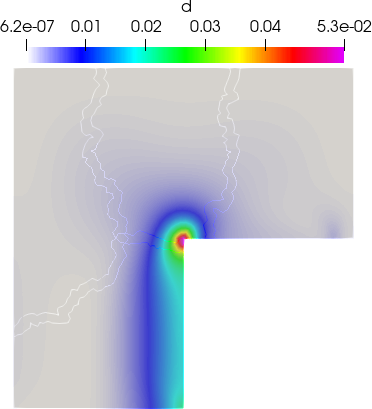
\includegraphics[width=0.3\textwidth]{./Images/fm-d1.png}
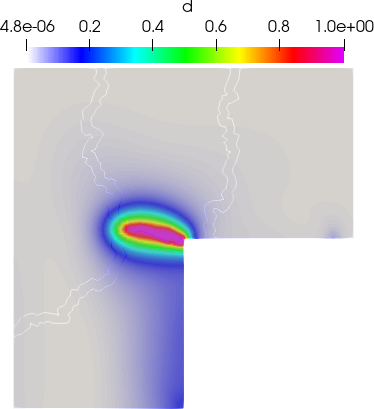
\includegraphics[width=0.3\textwidth]{./Images/fm-d2.png}
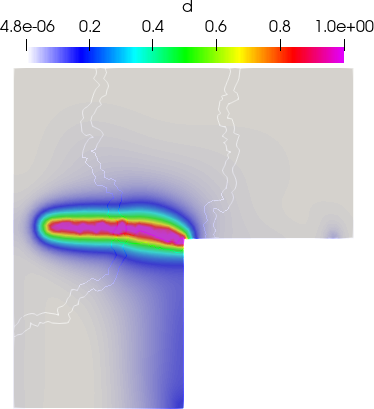
\includegraphics[width=0.3\textwidth]{./Images/fm-d3.png}
\caption{Finite element solution showing: Crack initiation,  movement, and  development. \label{L-shape-mesh-crack}}
\end{figure}

On you screen, the force displacement curve which plots \psd{force.data}
should look something like this

\begin{figure}[h!]
\centering
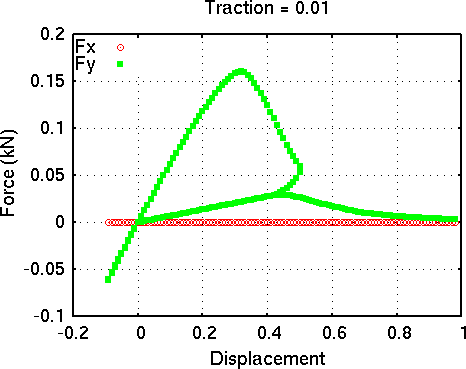
\includegraphics[width=0.5\textwidth]{./Images/fm-force-displacement.png}
\caption{Force-displacement curve with cyclic loading. \label{L-shape-fd-curve}}
\end{figure}
